\documentclass[10pt]{article}
\usepackage[paperwidth=40in, paperheight=40in]{geometry}
\usepackage[usenames]{color} %used for font color
\usepackage{amssymb} %maths
\usepackage{amsmath} %maths
\usepackage[utf8]{inputenc} %useful to type directly diacritic characters

%%% Sans serif text font
\usepackage[scaled]{helvet}
\renewcommand*\familydefault{\sfdefault}\usepackage[T1]{fontenc}
%%%

\usepackage{skull}
\usepackage{tikz}
\usetikzlibrary{positioning}
\usetikzlibrary{arrows}
\usetikzlibrary{fit}
\usetikzlibrary{calc}
\usetikzlibrary{automata}
\usetikzlibrary{decorations.markings}
\usetikzlibrary{decorations.pathreplacing}

\tikzset{>=latex}
\tikzstyle{snode}=[black,draw=black,line width=1.5pt,shape=circle,fill=white,minimum size=8mm]
\tikzstyle{obnode}=[black,draw=black,line width=1.5pt,shape=circle,fill=black!20!white,minimum size=8mm]
\tikzstyle{detnode}=[black,draw=black,line width=1.5pt,densely dotted,shape=circle,fill=white,minimum size=8mm]
\tikzstyle{constnode}=[black,draw=black,line width=1.5pt,shape=rectangle,fill=white,minimum size=8mm]
\tikzstyle{mincnode}=[black,draw=black,line width=0.75pt,shape=rectangle,fill=white,minimum size=3mm]
\tikzstyle{blnode}=[white,draw=black,line width=1pt,shape=circle,fill=black,minimum size=1mm,font=\scriptsize,inner sep=1pt]
\tikzstyle{ylnode}=[black,draw=black,line width=1pt,shape=circle,fill=yellow,minimum size=1mm,font=\scriptsize,inner sep=1pt]
\tikzstyle{taro}=[->,line width=2pt,color=black]
\tikzstyle{thintaro}=[->,line width=0.75pt,color=black]
\tikzstyle{dtaro}=[->,line width=2pt, densely dotted,color=black]
\tikzstyle{smod}=[black, draw=black, line width=2pt, fill=white, shape=rectangle, rounded corners, minimum size=10mm, minimum width=20mm]
\tikzstyle{obmod}=[black, draw=black, line width=2pt, fill=black!20!white, shape=rectangle, rounded corners, minimum size=10mm, minimum width=20mm, minimum width=20mm]

\definecolor{shc}{RGB}{238,224,229}
\definecolor{shc2}{RGB}{182,152,195}
\definecolor{brnt}{RGB}{221,132,13}

\begin{document}
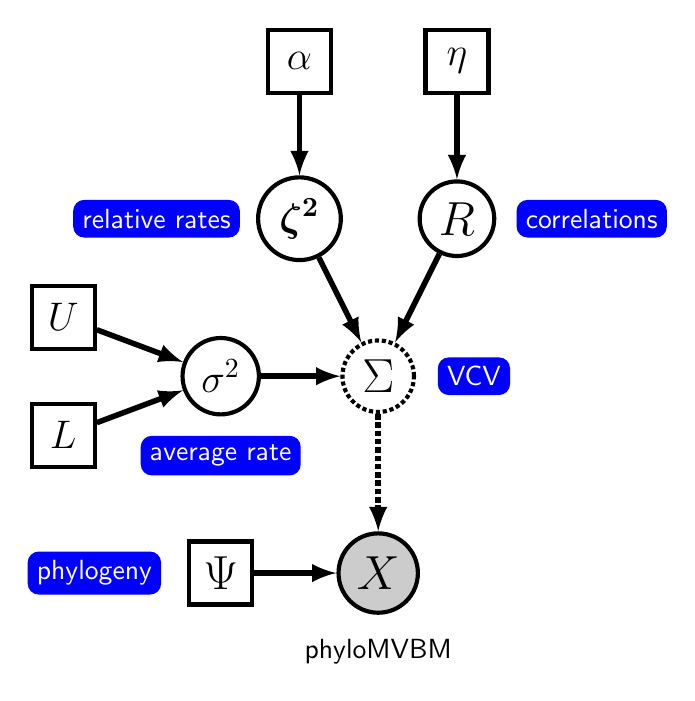
\begin{tikzpicture}
\node[obnode] (nx) at (1,1) {\LARGE $X$};
\node[constnode] (phylo) at ($(nx)+(-2,0)$) {\LARGE $\Psi$};
\node[detnode] (sigma) at ($(nx)+(0,2.5)$) {\LARGE $\Sigma$};
\node[snode] (ar) at ($(sigma)+(-2,0)$) {\Large $\sigma^2$};
\node[snode] (rr) at ($(sigma)+(-1,2)$) {\Large $\boldsymbol{\zeta^2}$};
\node[snode] (cr) at ($(sigma)+(1,2)$) {\LARGE $R$};
\node[constnode] (alpha) at ($(rr)+(0,2)$) {\Large $\alpha$};
\node[constnode] (eta) at ($(cr)+(0,2)$) {\Large $\eta$};
\node[constnode] (u) at ($(ar)+(-2,0.75)$) {\Large $U$};
\node[constnode] (l) at ($(ar)+(-2,-0.75)$) {\Large $L$};
\draw [taro] (phylo) -- (nx);
\draw [dtaro] (sigma) -- (nx);
\draw [taro] (ar) -- (sigma);
\draw [taro] (rr) -- (sigma);
\draw [taro] (cr) -- (sigma);
\draw [taro] (alpha) -- (rr);
\draw [taro] (eta) -- (cr);
\draw [taro] (l) -- (ar);
\draw [taro] (u) -- (ar);
\node at ($(nx)+(0,-1)$) {phyloMVBM};
\node[white, fill=blue, shape=rectangle, rounded corners] at ($(phylo)+(-0.75,0)$) [left]{phylogeny};
\node[white, fill=blue, shape=rectangle, rounded corners] at ($(ar)+(0,-0.75)$) [below]{average rate};
\node[white, fill=blue, shape=rectangle, rounded corners] at ($(sigma)+(0.75,0)$) [right]{VCV};
\node[white, fill=blue, shape=rectangle, rounded corners] at ($(rr)+(-0.75,0)$) [left]{relative rates};
\node[white, fill=blue, shape=rectangle, rounded corners] at ($(cr)+(0.75,0)$) [right]{correlations};
\end{tikzpicture}
\end{document}